\section*{Lezione 13}
\addcontentsline{toc}{section}{Lezione 13}

Abbiamo detto che la capacità è difficile da calcolare perchè dipende dalla distribuzione dei simboli di ingresso e di uscita (che poi dipendono da quelli in entrata).\\
Quindi abbiamo detto magari ci sono dei canali in cui questi conti sono più semplici: i canali uniformi.\\
La matrice di questi canali contiene righe che sono l'una la permutazione dell'altra, ad esempio il canale binario simmetrico:
\begin{equation*}
\begin{pmatrix}
P & Q\\
Q & P
\end{pmatrix}
\end{equation*}
Perchè il canale uniforme ci semplifica il conto? Perchè la mutua informazione del sistema può essere scritta come:
\begin{equation*}
I(A;B)= H_r(B)-H_r(B\,|\,A) = H_r(B) - \sum_{A}\sum_{B}P(a,b)\log_r\frac{1}{P(B\,|\,A)}
\end{equation*}
\begin{equation*}
= H_r(B) - \sum_{A}p(a)\underbrace{\sum_{B}P(b\,|\,a)\log_r\frac{1}{P(b\,|\,a)}}_{\text{*}}
\end{equation*}

Andiamo a considerare la sommatoria (*), noi stiamo considerando la matrice di canale (dove ogni cella è $p(b\,|\,a)$), quindi il primo termine della somma, ci stiamo muovendo su una riga fissata (quella $a_i$).\\
Dato che il canale è uniforme, il risultato su ogni riga è uguale in quanto ogni riga è una permutazione dell'altra (li sommo solo in ordine differente).
Diciamo che:
\begin{equation*}
w = \sum_{B}P(b\,|\,a)\log_r\frac{1}{P(b\,|\,a)} = H_r(B\,|\,a)
\end{equation*}
Quindi $w$ ha un valore fissato che è uguale per tutte le righe e non dipende da $a$, quindi ottengo:
\begin{equation*}
= H_r(B) - w \sum_{A}p(a)
\end{equation*}
\begin{equation*}
= H_r(B) - w = I(A;B)
\end{equation*}

e questo è più è semplice da calcolare rispetto a $H_r(B)-H_r(B\,|\,A)$.

Facciamo un esempio con un canale binario simmetrico. 
\begin{equation*}
\begin{pmatrix}
P & Q\\
Q & P
\end{pmatrix}
\end{equation*}
La capacità è uguale a $H_2(B) - w$ dove
\begin{equation*}
w = P\log_2\frac1P+Qlog_2\frac1Q = 
\end{equation*}
\begin{equation*}
= P\log_2\frac1P+(1-P)log_2\frac{1}{1-P} = H_2(P)
\end{equation*}
\begin{equation*}
= Q\log_2\frac{1}{1-Q}+Qlog_2\frac{1}{Q} = H_2(Q)
\end{equation*}

Entrambi i valori sono uguali all'entropia di una bernoulliana.
\begin{equation*}
I(A;B)=H_2(B) - H_2(P)=H_2(B) - H_2(Q)
\end{equation*}
Ricordiamo che
\begin{equation*}
C=max(H_2(B)-H_2(P))
\end{equation*}
Siccome $H_2(P)$ è una costante, occupiamoci sono di massimizzare $H_2(B)$. Abbiamo già visto che questa funzione ha valore massimo 1 quanto $x=\frac12$. Quanto è però il valore di $p$ tale per cui $H_2(B)$ ha come $x=\frac12$?
\begin{equation*}
x = \frac12 = pP + (1-p)Q
\end{equation*}
\'E quindi la probabilità che venga mandato un 0 e arrivi uno 0 più la probabilità che venga mandato 1 e arrivi 0.
\begin{equation*}
= pP + (1-P)-p(1-P)
\end{equation*}
\begin{equation*}
 = 1-P-p + 2pP
\end{equation*}
\begin{equation*}
= 1 - P - p(1 - 2P)
\end{equation*}
\begin{equation*}
\downarrow
\end{equation*}
\begin{equation*}
p(1-2P) = \frac12 - P
\end{equation*}
\begin{equation*}
p\cancel{(1-2P)} = \frac{\cancel{1-2P}}{2}
\end{equation*}
Posso semplificare in quanto $(1-2P) = 0$ solo in caso di $P=\frac12$ e quindi di canale totalmente rumoroso.
\begin{equation*}
p = \frac{1}{2}
\end{equation*}

Quindi esiste un valore di $p$ che mi consente di ottenere $x=\frac12$ per cui $H_2(B)$ ottiene valore massimo, quindi ho che:

\begin{equation*}
C = 1 - H_2(P)
\end{equation*}
\begin{equation*}
C = 1 - H_2(Q)
\end{equation*}

\newpage
\subsection*{Secondo teorema di Shannon}
\addcontentsline{toc}{subsection}{Secondo teorema di Shannon}
Questo teorema mette insieme tutto quello che abbiamo detto, cioè raccoglie cosa vuol dire fare trasmissioni all'interno di un canale rumoroso applicando codici a correzione d'errore e cercando di sfruttare il canale al miglior modo possibile, quindi cercando di avvicinarsi al più possibile alla capacità di canale.

\begin{theorem}
	Dato un canale rumoroso è sempre possibile avvicinarsi in maniera arbitraria alla capacità del canale mantenendo contemporaneamente arbitrariamente bassa la probabilità d'errore.
\end{theorem}

Quindi abbiamo un canale rumoroso, e questo canale ha una certa capacità (il massimo al variare delle $p(a)$ della mutua informazione del sistema).\\
Questo teorema dice che è possibile avvicinarsi arbitrariamente al valore della capacità (tipo asintoto). Avvicinarsi vuol dire trovare delle codeword, o una codifica, per cui ci si avvicina.
\medskip
Avvicinandomi alla capacità del canale inserisco sempre più informazione, e mandandone sempre di più ovviamente sbaglia sempre di più, e sbagliando di più si aumenta la probabilità che il ricevente sbagli a correggere una codeword (due errori e si corregge male).

La \textbf{5} si riferisce alla probabilità che il ricevente \textit{corregga male} una codeword.

\subsection*{Dimostrazione - Secondo teorema di Shannon}
\addcontentsline{toc}{subsection}{Dimostrazione - Secondo teorema di Shannon}
\subsubsection*{Preliminari matematici:}
\addcontentsline{toc}{subsubsection}{Preliminari matematici}
\begin{itemize}
	\item \begin{equation*}
	\sum_{k=0}^{\lambda n}\binom{n}{k} \leq 2^{nH(\lambda)} \; \; \; \;\; \text{per } 0 < \lambda < 1 \; \; \; \; \text{e } \lambda n \text{ intero}
	\end{equation*}
	
	Dove $H(\lambda)$ è l'entropia di una sorgente bernoulliana con due simboli di probabilità $\lambda$ e $1-\lambda$.
	
	\item Legge debole dei grandi numeri:\\
	Supponiamo di avere $n$ variabili casuali indipendenti fra loro ($x_1, x_2, ..., x_n$) tutte con la stessa distribuzione di probabilità caratterizzata da media $\mu$ e varianza $\sigma^2$.\\
	Allora abbiamo che per ogni $\epsilon > 0$ e per ogni $\delta> 0$ esiste un interno $n_0$ tale che per ogni $n\geq n_0$ vale che:
	\begin{equation*}
	P(|\frac1n\sum_{i=1}^nX_i-\mu| \leq \epsilon) \geq 1 - \delta
	\end{equation*}
	oppure in maniera equivalente:
	\begin{equation*}
	P(|\frac1n\sum_{i=1}^nX_i-\mu| > \epsilon) < \delta
	\end{equation*}
	
	Notiamo che $\frac1n\sum_{i=1}^nX_i$ è la media campionaria dei miei $n$ esperimenti, mentre $\mu$ è la media teorica.
	Quindi sottraendoli in valore assoluto mi chiedo quanto sono distanti (teoria e pratica).\\
	La probabilità che questa distanza superi un valore $\epsilon$ piccolo a piacere può essere resa piccola a piacere $\delta$.\\
	Nel nostro caso ogni esperimento sarà l'invio di un bit all'interno di un canale binario simmetrico.\\
	Metto $n$ copie del canale binario simmetrico ($n$-esima estensione) indipendenti fra loro, quindi la probabilità teorica di ottenere errori è $Qn$ ($\mu$).
	\smallskip
	
	In pratica inviare pacchetti tramite $n$-esima estensione CDS ($\text{CDS}^n$) equivale a trasmettere pacchetti di $n$ bit col modello del rumore bianco.\\
	
	Assumeremo che $Q < \frac12$ (se fosse maggiore metto una porta \texttt{not}, se uguale ho canale completamente rumoroso).
	
	\item Regola di decisione: essa è la regola/funzione che il ricevente applica per cercare di capire quale secondo lui è il simbolo che è stato spedito. Esempio (probabilita all'indietro $P(a_i\,|\,b_j)$):

	\[
	\kbordermatrix{
		& b_1 & b_2 & b_3 \\
		a_1 & 0.6 & 0.5 & 0.4 \\
		a_2 & 0.4 & 0.5 & 0.6
	}
	\]
	
	Assumiamo che la distribuzione delle $a_i$ sia uniforme, quindi $p(a_1) = p(a_2) = \frac12$.\\
	
	La funzione di decisione di massima verosimiglianza $d:B\rightarrow A$ è definita in queto modo:
	\begin{itemize}
		\item $d(b_1) = a_1$
		\item $d(b_3) = a_2$
		\item $d(b_2) = a_1 \lor d(b_2) = a_2$		
	\end{itemize} 

	Da notare come questa regola non abbia un unico risultato ($b_2$).
	La regola di verosimiglianza funzione in questo modo:
	\begin{equation*}
	d(b_j) = a^* \;\;\; \text{t.c.} \;\;\; P(a^*\,|\,b_j) \geq P(a_i\,|\,b_j) \; \; \forall i
	\end{equation*}
	Applicando Bayes sto dicendo che:
	\begin{equation*}
	\frac{p(b_j\,|\,a^*)p(a^*)}{\cancel{p(b_j)}} \geq \frac{p(b_j\,|\,a_i)p(a_i)}{\cancel{p(b_j)}}
	\end{equation*}
	Abbiamo detto che, non sapendo a priorio la distribuzione dei simboli di ingresso, assumo che sia uniforme; quindi:
	\begin{equation*}
	p(b_j\,|\,a^*)\cancel{\frac1q} \geq p(b_j\,|\,a_i)\cancel{\frac1q}
	\end{equation*}
	\begin{equation*}
	p(b_j\,|\, a^*) \geq p(b_j\,|\,a_i)
	\end{equation*}
	
	\item Capacità di un $\text{CBS}^n$: $n \times C$, dove $C=n(1-H_2(P)) = n(1-H_2(Q))$
\end{itemize}

\subsubsection*{Dimostrazione:}
\addcontentsline{toc}{subsubsection}{Dimostrazione}
N.B. $a_i$ e $b_j$ sono pacchetti di $n$ bit.\\
I messaggi validi fra tutte le $n$-ple di bit di A è $|A|=M\leq 2^n$. Diciamo inoltre che sono equiprobabili, quindi $p(a_i) = \frac1M$, quindi la quantità di informazione $I(a_i) = \log_2\frac{1}{\frac1M} = \log_2M$.\\
Il nostro obiettivo è quello di avvicinarci alla capacità del canale, che è:
\begin{equation*}
\text{Capacità CBS}^n = n \times C
\end{equation*}
Scelgo un $\epsilon_1 > 0$ piccolo a piacere, e chiedo che la quantità di informazione si avvicini per meno di una quantità proporzionale a $\epsilon_1$ alla capacità, quindi:
\begin{equation*}
I(a_i)=nC - \epsilon_1
\end{equation*}
Anche se in realtà questa $\epsilon_1$ dovrebbe funzionare (è più \textit{fair}) in relazione al numero di estensioni $n$, quindi:
\begin{equation*}
I(a_i)=n(C - \epsilon_1)
\end{equation*}
Da questa relazione possiamo ricavare $M$:
\begin{equation*}
M = 2^{n(C-\epsilon_1)} = \frac{2^{nC}}{2^{n\epsilon_1}}
\end{equation*}

Ora mettiamoci nei panni del ricevente: una volta ricevuto $b_j$ si costruisce una iper-sfera centrata in $b_j$ e avrà un raggio lungo $nQ$ in quanto mi aspetto $nQ$ errori.
Ora osservo che $b_j$ non sia un codice valido, quindi devo scegliere il messaggio più vicino a $b_j$ all'interno della sfera.

\begin{figure}[h]
	\centering
	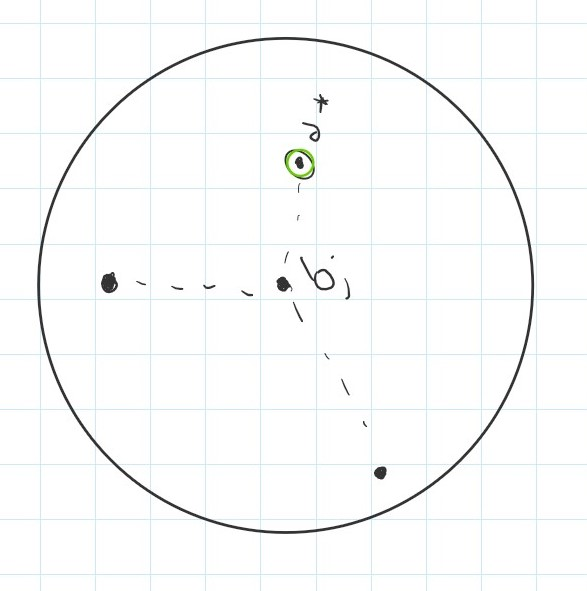
\includegraphics[width=0.45\linewidth]{immagini/img30}
\end{figure}

Quindi, data la distanza D fra $b_j$ e $a^*$ la probabilità
\begin{equation*}
p(b_j\,|\,a^*) = Q^D(1-Q)^{n-D}
\end{equation*}
per $Q < \frac12$ è decrescente al crescere di $D$, quindi la probabilità che ottenga questo $b_j$ da $a_i$ è tanto più bassa quanto sono lontani $a_i$ e $b_j$, quindi la distanza non è solo topologica.\\
In altre parole scelgo una $a^*$ che mi minimizza questa quantità: $Q^D(1-Q)^{n-D}$.\\
Il problema è che può essere complicato trovare quello più vicino e che può esserci una $a^*$ che ha la stessa distanza fra due $b_j$ (le regole di massima verosimiglianza non sono uniche).




